%& -shell-escape -enable-write18
\documentclass{standalone}
\usepackage{tikz}
\usetikzlibrary{external}
%\tikzexternalize
\usetikzlibrary{shapes,arrows}
\usepackage{caption}
\usetikzlibrary{matrix}
%\newcommand{mynodename}[#1]{\mathrm{#1}}\label{•} 
%\newcommand{mylabelleft}[#2]{label={[font=\fontsize{#1}{#1}\selectfont]above left:mynodename{#2}}}

\begin{document}
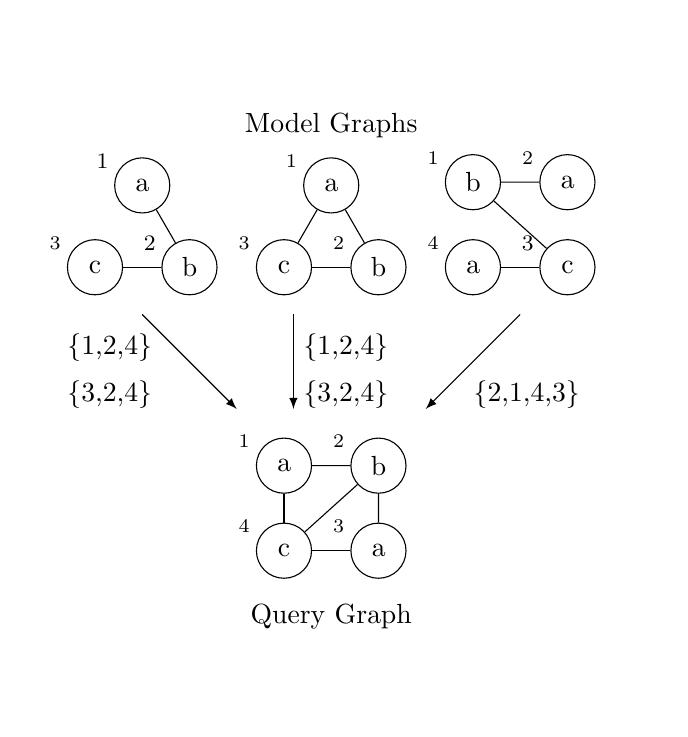
\begin{tikzpicture}[scale=1.2]
%[every node/.style={draw,circle}]
\tikzstyle{every node}=[draw,shape=circle,minimum size=0.7cm];
\tikzstyle{line} = [draw,-latex]
\colorlet{invisible}{white}
\colorlet{visible}{black}
%\tikzstyle{mylabelsfont=[font=\fontsize{7}{7}\selectfont,yshift=-.2cm];
%\tikzstyle{every label}=[text height=10pt];
\begin{scope}[shift={(0,-0.5)}] 
	\begin{scope}[yshift=0cm]% top row as a group
%	\draw[help lines] (-1,-6) grid (10,6);
	  \node (a) at (60:1cm) [label={[font=\fontsize{8}{8}\selectfont,yshift=-.2cm]above left:$1$}] {a};
	  \node (b) at (0:1cm)  [label={[font=\fontsize{8}{8}\selectfont,yshift=-.2cm]above left:$2$}] {b};
	  \node (c) at (0:0cm)  [label={[font=\fontsize{7}{7}\selectfont,yshift=-.2cm]above left:$3$}] {c};
	
	  \foreach \from/\to in {c/b,b/a}
	    \draw (\from) -- (\to);
	\end{scope}
	\begin{scope}[xshift=2cm]%top row middle
	  \node (a) at (60:1cm) [label={[font=\fontsize{7}{7}\selectfont,yshift=-.2cm]above left:$1$}] {a};
	  \node (b) at (0:1cm)  [label={[font=\fontsize{7}{7}\selectfont,yshift=-.2cm]above left:$2$}] {b};
	  \node (c) at (0:0cm)  [label={[font=\fontsize{7}{7}\selectfont,yshift=-.2cm]above left:$3$}] {c};
	
	  \node [draw=none] (query_label) at (0.5,1.5) {Model Graphs};% Model label
	  \foreach \from/\to in {c/b,b/a,c/a}
	    \draw (\from) -- (\to);
	\end{scope}
	\begin{scope}[xshift=4cm]%top row right
	  \node (a_1) at (0,0) [label={[font=\fontsize{7}{7}\selectfont,yshift=-.2cm]above left:$4$}] {a};
	  \node (b) at (0,.9)  [label={[font=\fontsize{7}{7}\selectfont,yshift=-.2cm]above left:$1$}] {b};
	  \node (c) at (1,0)   [label={[font=\fontsize{8}{8}\selectfont,yshift=-.2cm]above left:$3$}] {c};
	  \node (a_2) at (1,.9) [label={[font=\fontsize{7}{7}\selectfont,yshift=-.2cm]above left:$2$}] {a};
	
	  \foreach \from/\to in {a_1/c,c/b,b/a_2}
	    \draw (\from) -- (\to);
	\end{scope}
\end{scope}
\begin{scope}[shift={(0,0)}] % The arrow and bracket as a group
	\begin{scope}[shift={(0,-0.5)}]%just the arrows
		\path[line] (0.5,-0.5) -- (1.5,-1.5);
		\path[line] (2.1,-0.5) -- (2.1,-1.5);
		\path[line] (4.5,-0.5) -- (3.5,-1.5);
	\end{scope}
	\begin{scope}[shift={(0.5,-1.6)}]%annotations at left arrow
		\matrix (m)[matrix of nodes, column  sep=-1mm,color=visible,row  sep=-1mm, anchor=center,draw=none, nodes={rectangle,color=invisible,draw=none,text width = 2cm} ]{
\node [color=visible] {\{1,2,4\}};&\\
\node[color=visible]{\{3,2,4\}};& \\
};
	\end{scope}
	\begin{scope}[shift={(3.0,-1.6)}]%%annotations at middle arrow
	\matrix (m)[matrix of nodes, column  sep=-1mm,color=visible,row  sep=-1mm, anchor=center,draw=none,nodes={rectangle,color=invisible,draw=none,text width = 2cm} ]{
\node [color=visible] {\{1,2,4\}};&\\
\node[color=visible]{\{3,2,4\}};& \\
	};
	\end{scope}
	\begin{scope}[shift={(4.8,-1.6)}]%%annotations at right arrow
	\matrix (m)[matrix of nodes, column  sep=-1mm,color=visible,row  sep=-1mm, anchor=center,draw=none,nodes={rectangle,color=invisible,draw=none,text width = 2cm} ]{
\node [color=visible] {};&\\
\node[color=visible]{\{2,1,4,3\}};& \\
	};
	\end{scope}
\end{scope}

\begin{scope}[shift={(2,-3.5)}]%bottom row graph
  \node (a_3) at (1,0) [label={[font=\fontsize{7}{7}\selectfont,yshift=-.2cm]above left:$3$}] {a};
  \node (b) at (1,.9)  [label={[font=\fontsize{7}{7}\selectfont,yshift=-.2cm]above left:$2$}] {b};
  \node (c) at (0,0)   [label={[font=\fontsize{7}{7}\selectfont,yshift=-.2cm]above left:$4$}] {c};
  \node (a_4) at (0,.9) [label={[font=\fontsize{7}{7}\selectfont,yshift=-.2cm]above left:$1$}] {a};
  
  \node [draw=none] (query_label) at (.5,-.7) {Query Graph};% query graph label
  \foreach \from/\to in {a_3/c,a_3/b,c/b,c/a_4,b/a_4}
    \draw (\from) -- (\to);
    
\end{scope}
\end{tikzpicture}
\end{document}